\documentclass{sig-alternate-05-2015}
\usepackage{hyperref}
\usepackage{graphicx}
\usepackage{amsmath}
\usepackage{csquotes}
% \usepackage{caption}
\usepackage{apacite}
\usepackage[letterpaper, portrait, margin=1in]{geometry}

\title {Final Paper, CS6460 (Educational Technology)}
\date{July 30, 2017}
\author{Chris Hodapp,
  \href{mailto:chodapp3@gatech.edu}{\nolinkurl{chodapp3@gatech.edu}}}

\begin{document}

\maketitle

\begin{abstract}
  Many programming languages or environments have been created for the
  purpose of teaching programming interactively (such as Logo,
  Scratch, Processing, and Squeak), and have at their root Papert's
  notion of constructionism.  At the same time, the web browser has
  become an increasingly common mode of delivery of technical
  tutorials and even textbook content, and accomodates increasingly
  sophisticated content to the point of that content not just
  including full graphical programs, but being a development platform
  in its own right.  The project described here is an attempt to
  combine these in some fashion.  More specifically, it presents an
  interactive 2D/3D programming and rendering environment via WebGL,
  uses this environment as a platform for content designed to teach
  some topics in mathematics, and delivers all of this via online
  content accessible from most contemporary web browsers.  It is
  presently hosted online at
  \url{https://hodapp87.github.io/cs6460_project}.
\end{abstract}

\section{Introduction}

Computer programming has been used as a platform for teaching various
subjects as computers became more and more widespread.  The most
notable example of this is perhaps via Seymour Papert's work in
constructionism and his co-creation of the Logo programming language
for teaching mathematics and analytical thought, primarily to
children\cite{Stager2016,Papert:1993,Papert:1980,Papert1999}.  His
approach here stresses the importance in education of the learner
being empowered to build things and being able to ``see'' from the
perspective of some abstraction (such as the turtle in Logo) as a way
of guiding and honing intuition.

Resnick, reflecting on the design of the
\href{https://scratch.mit.edu/}{Scratch} language and its roots in
Logo, also offers a succint summary \cite{Resnick2009} of the
balancing act of creating a programming language whose goal is to
educate:

\blockquote{Papert argued that programming languages should have a
  ``low floor'' (easy to get started) and a ``high ceiling''
  (opportunities to create increasingly complex projects over
  time). In addition, languages need ``wide walls'' (supporting many
  different types of projects so people with many different interests
  and learning styles can all become engaged). Satisfying the triplet
  of low-floor/high-ceiling/wide-walls hasn't been
  easy.}

The same author also gives a reason why one should use programming at
all in teaching:

\blockquote{The ability to program provides important benefits. For
  example, it greatly expands the range of what you can create (and
  how you can express yourself) with the computer. It also expands the
  range of what you can learn. In particular, programming supports
  ``computational thinking,'' helping you learn important
  problem-solving and design strategies (such as modularization and
  iterative design) that carry over to nonprogramming domains. And
  since programming involves the creation of external representations
  of your problem-solving processes, programming provides you with
  opportunities to reflect on your own thinking, even to think about
  thinking itself.}

% Model progression

In a somewhat related way, web content has made up a substantial
amount of learning material, including at the same scope as a
textbook.  Some more-established examples of this are SICP (Structure
and Interpretation of Computer Programs)\cite{SICP}, HtDP (How to
Design Programs)\cite{HTDP}, and Software Foundations\cite{SF}.
Overall, though, these are still something like ``traditional''
textbook content distributed in a way that takes advantage of
electronic media in general, but does not make any particular use of
the nuances of web content or the web browser.  Software Foundations,
which teaches principles of computation and formal proofs using the
Coq programming language, applies a notable method here: the learner
can read the entire book in the Coq environment, and examples and
exercises are provided in the form of Coq code which can be edited,
compiled, and evaluated directly in that environment.  SICP and HtDP
have both been used in introductory computer science courses at
colleges, including ``traditional'', non-online
courses\cite{Felleisen,WhySICP}.

At the same time, web browsers have also progressed substantially from
their original purpose of accessing content.  At the present, the web
browser is a platform unto itself for running applications (via
JavaScript), and these applications can be quite sophisticated: they
may be written in many other programming languages (provided the
language can compile to JavaScript), they may be highly visual and
interactive with the help of things like Canvas and SVG and use
hardware-accelerated 3D graphics by way of WebGL, these applications
may even be development environments unto themselves (due to
JavaScript's interpreted nature), and presently the majority of
browsers across both desktop computers and mobile devices support all
of these features simply as standard.

Learning material has made some good use of this; for instance,
\href{http://setosa.io/ev/eigenvectors-and-eigenvalues/}{Eigenvectors
  and Eigenvalues Explained Visually} and
\href{http://students.brown.edu/seeing-theory/index.html}{Seeing
  Theory: A visual introduction to probability and statistics} made
use of the visual capabilities of web browsers to present topics in
mathematics.  While this is not anything new per se (similar things
are numerous in the form of desktop applications, Java applets, Flash
applications, and mobile applications), these have the advantage that
they can run nearly anywhere a modern web browser does and typically
without requiring any special configuration, plugins, or other
software.

For interactive learning materials for programming education, one
common paradigm is that the web browser is used as an interface for
resources that are mostly hosted server-side (typically, an
implementation of some programming language), as technologies like
Ajax made more feasible around 2005\cite{Ajax}. For instance, with the
\href{https://golang.org/}{Go programming language interactive
  tutorial}, the user edits the Go program in the browser, and the
interface then submits the code to a server which is responsible for
compiling it, executing it, and submitting the results back to the
browser.  While this is a very flexible method, it has drawbacks:

\begin{itemize}
\item It requires that the server have the right software,
  configuration, and resources to host the environment in question.
\item It may require a reasonably fast Internet connection, or at
  least a low-latency one, for the interface to be usable.  For any
  larger amount of data that the code is to handle - such as images,
  audio, or video - this can be problematic.
\item Users are given the freedom to run arbitrary programs on a
  remote server, and the server must be equipped to prevent accidental
  or malicious misuse from causing problems.  For instance, a user
  should not be able to delete or even access arbitrary files on the
  server, access privileged system calls, use all available memory or
  disk space, or indefinitely run a program that occupies a large
  amount of resources.  This ranges between difficult and impossible
  to enforce at the language level, and as a result servers will
  commonly employ some kind of virtualization or other sandboxing to
  try to achieve this.
\end{itemize}

However, as mentioned, the web browser is able to run JavaScript code,
and this ability has become increasingly sophisticated.  One obvious
use of this is that content can allow the learner to edit, debug, and
execute JavaScript code directly in their browser (and indeed most
browsers come built-in with development tools to this end) - such as
\href{https://jsfiddle.net/}{JSFiddle}.  This has various benefits:
the sandboxed nature of the browser prevents the learner from doing
any real damage, the fact that the code only executes on one's own
computer limits that damage further (as the sandboxing is never
perfect), and any language implementation that compiles to JavaScript
can be run in the browser.  Tools such as
\href{http://emscripten.org/}{Emscripten} from Mozilla extend the
reach of this considerably.

As an example of this, the Lean Theorem Prover has several tutorials
(such as \cite{LeanIntro}) which are implemented in much the same way
as Software Foundations, but hosted completely in the web browser.
The fact that they could compile the implementation of the Lean
language itself to JavaScript (that is, its compiler and runtime run
directly in the browser) enabled them to host in this way without
requiring any particular server-side resources.  However, the user is
not required to run this way; Lean is still available as a
natively-compiled application or as source code.

The visual programming language
\href{https://processing.org/}{Processing} - itself designed for
teaching programming visually\cite{P5Design} - provides another
example of this with in the form of
\href{https://processingjs.org/}{Processing.js}, a version of
Processing ported to JavaScript.

Programming using tooling outside of the web browser (e.g. in a
dedicated IDE, using a text editor and some commandline tools, or at a
REPL) is still a superior option for many contexts, particularly for
programming tasks that are lower-level, more performance-critical, or
more complex.  However, these almost always come with some sort of
barrier to entry that is in addition to the difficulty of learning the
language in the first place: the tooling must be installed, sometimes
licenses must be acquired, the tooling often has an interface with its
own nuances that must be learned, and the tooling may require separate
installation or management of plugins, libraries, packages, and so on.

These approaches are not necessarily exclusive of each other though.
Environments based in the web browser can provide a sort of ``low
floor'' here (as in the Papert quote), but can achieve the ``high
ceiling'' and ``wide walls'' part of things by making it more feasible
for the user to transition to more dedicated tools when needed.

\section{Goals}

In light of the current context of web browsers and their
capabilities, the goal in this project was to create educational
content, and an interactive programming environment, along the
following lines:

\begin{itemize}
\item The content is hosted inside of an interactive programming
  environment which can run from a web browser, ideally with minimal
  server requirements (i.e. 
\item Content and implementation should be freely available as
  open source.
\item The interactive programming environment is sufficient to allow
  the user most of the ``normal'' amenities in a language, includes
  built-in functionality for creating graphics, visualizations, and
  animation, and is advanced enough to accomodate some sophistication
  here (for instance, a raytracer or other 3D renderer).
\item Content is directed at letting the learner explore topics in
  analytic geometry and linear algebra by way of writing programs
  which create graphics.
\end{itemize}

The content's area is something of a subtlety: It is not meant as
introductory programming lessons, nor as a tutorial in how to create
graphics or how to write a renderer, nor as solely mathematical
content. It is meant as an explanation of some mathematical topics,
using interactive programming of graphics as the method.

This was based partly around Papert's notion of making math
``appropriable'': \blockquote{In many ways mathematics - for example
  the mathematics of space and movement and repetitive patterns of
  action - is what comes most naturally to
  children.}\cite{Papert:1993} While the content isn't meant for
children, but for younger adults with some existing programming and
mathematics experience, the principle should hold similarly.

% The web is the platform; it's used here to lower barriers to entry
% that can be considerable for people whose programming experience is
% limited.

\section{Implementation \& Content}

Everything discussed below is available to use at
\url{https://hodapp87.github.io/cs6460_project} and the source code
for this is at \url{https://github.com/hodapp87/cs6460_project}.

\subsection{Environment}

% TODO: What is the source code's license?

This is based on a modified version of
\href{https://github.com/leanprover/mkleanbook}{mkleanbook}, an open
source tool which is also the tool used to generate the
\href{https://leanprover.github.io/introduction_to_lean/}{Introduction
  to Lean} mentioned earlier (and other interactive Lean tutorials).

The modifications were primarily to replace the tool's support for the
Lean language with support more specific to WebGL.  WebGL support was
mostly done by integrating a modified version of
\href{https://github.com/gportelli/pocket.gl}{pocket.gl} which is
available at \url{https://github.com/Hodapp87/pocket.gl}; this
component was responsible for allowing the user to edit and render
WebGL code.

More specifically, the project includes a build process which turns
Emacs \href{http://orgmode.org/}{org-mode} markup into a webpage in
the form of a directory of static HTML/JavaScript/CSS that is suitable
for hosting directly from a web server.  This webpage contains content
produced from that org-mode markup, but it also contains an
interactive WebGL editor and renderer.  This org-mode markup can
contain segments of WebGL source code, and the build turns these into
properly-highlighted source code in the rendered page, placing a ``Try
code'' button below each segment which will transfer it directly to
the editor.

See figure \ref{fig:editor} for a screenshot showing an example of
this (from the content described in the next section) with the
Fragment Shader tab visible, and \ref{fig:render} for the same but
with the Render tab showing the animated result of some code (along
with its parameters).

Since everything was written to rely only on static files (and not
requiring any special server-side support), this page could be hosted
directly from its GitHub repository via
\href{https://pages.github.com/}{GitHub Pages}.  It does not rely on
anything specific to git or GitHub.

\begin{figure*}
  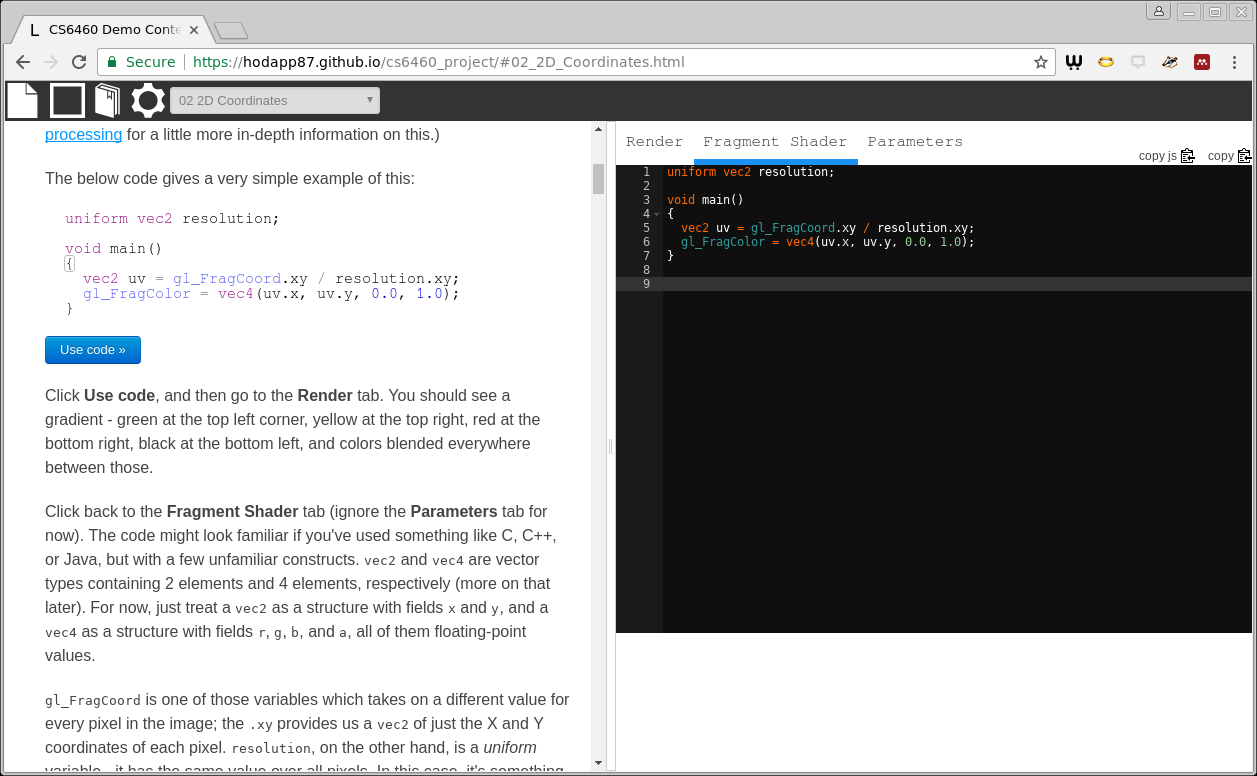
\includegraphics[width=\textwidth]{screenshot_editor.png}
  \caption{Project web page with Fragment Shader visible}
  \label{fig:editor}
\end{figure*}

\begin{figure*}
  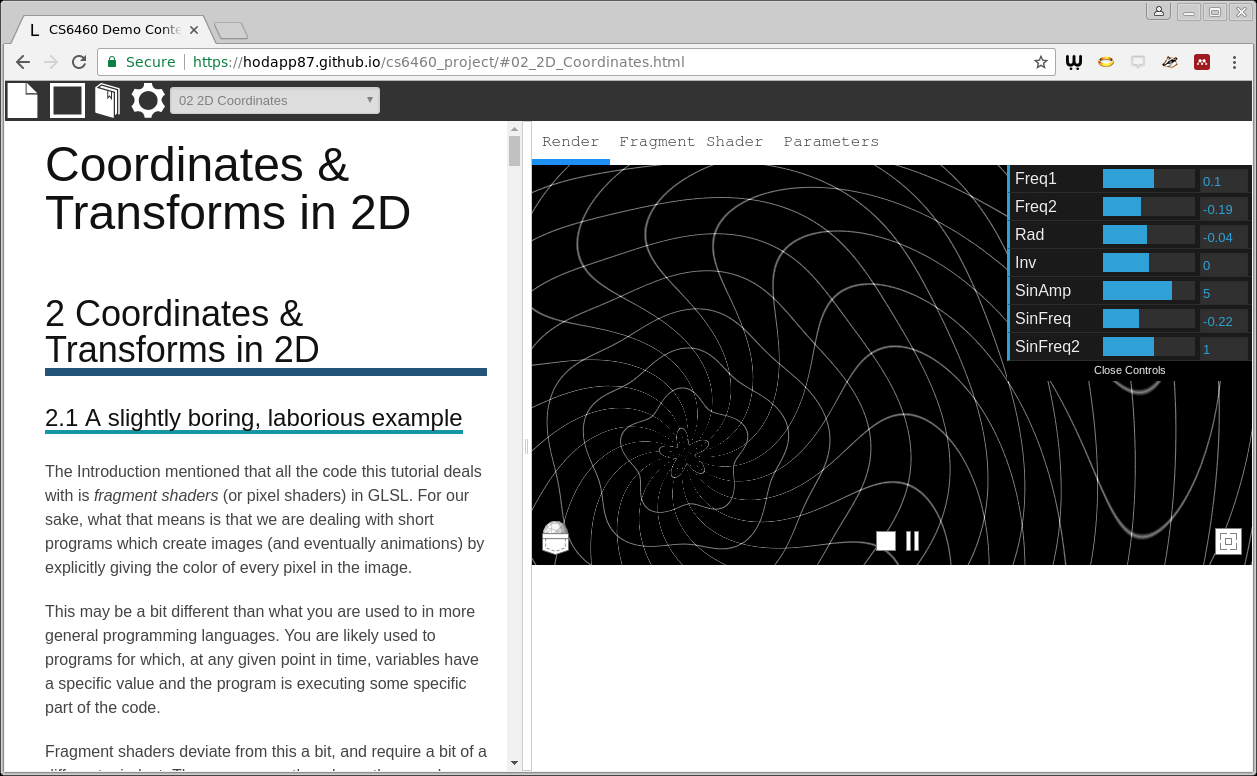
\includegraphics[width=\textwidth]{screenshot_render.png}
  \caption{Project web page with Render visible}
  \label{fig:render}
\end{figure*}

\subsection{Content}

The actual content of this project is done through the above
environment.  As planned, it tries to explain a small selection of
topics in mathematics using examples in WebGL which the learner may
execute and edit directly.

All code examples are implemented as standalone WebGL fragment
shaders.  That is, while the code can be hardware-accelerated, it uses
the GPU (if there is one) almost solely as a stream processor rather
than as dedicated rendering hardware, and so rather than focusing on
OpenGL's rendering model, it focuses on what can be done in creating
graphics pixel-by-pixel.

The main goal is in explaining and building intuition for the
mathematical topics in question.  A secondary goal is in empowering
the learner to still be working with ``real'' code and comprehending
its fundamental abstractions in such a way that it could easily be
applied in other places - such as a larger OpenGL application, a
homemade renderer, or any other shading language.

It is split into two main parts: a chapter with 2D graphics, and one
with 3D graphics.  The chapter on 2D graphics begins with creating
graphics using so-called functional images\cite{Elliott03:FOP} - that
is, an image that is produced by a function $f$ which maps an $(x,y)$
pixel location - a point in 2D space - to an RGB triplet,
i.e. $[0,1]^3$, to specify the color of pixel $(x,y)$.  The use of GL
fragment shaders is not incidental here: fragment shaders work exactly
according to this model.

The chapter walks through some mechanisms for working with the
coordinate space and drawing basic shapes under this model, and then
demonstrates how transforms applied to the domain of $f$ are
intuitively a sort of warping of space that can be comprehended
visually, and how function composition relates to this.  It also
explains some built-in functionality for being able to both animate
these graphics and interactively control parameters to them.

\enlargethispage{-\baselineskip}
\subsubsection{Sphere Tracing}

The next chapter presents one extension of this ``functional images''
model from 2D to 3D.  In specific, rather than a functions which
describes an image by mapping a 2D point $(x,y)$ to an RGB triplet, it
introduces \textrm{distance functions} which describe a 3D surface by
mapping a 3D point $(x,y,z)$ to the nearest distance from $(x,y,z)$ to
that surface (in other words, the radius $r$ of the largest sphere
located at $(x,y,z)$ which never intersects the surface).

One use of these distance functions is that raymarching can be used to
render them, and here a specific form of raymarching - sphere tracing
- is used
\cite{Hart,Hart1989,Quilez2008,Perlin1989,TexturingModelingText}.
An existing implementation of a sphere tracer from \'{I}\~{n}igo
Qu\'{i}lez is adapted for use in the example code.

Ray tracing is very commonly used in introducing a 3D renderer due to
the simplicity of implementation, however, sphere tracing is used
instead here because distance functions are much more flexible to the
sorts of transformations and deformations that are applied.  Figure
\ref{fig:sphere tracer} gives one simple example of a common effect
done in distance functions in a sphere tracer: CSG is used to create a
composite shape by subtracting a sphere from a cube, modulo is used to
tile the shape infinitely in all directions, and a variable rotation
is applied to this infinite field.

\begin{figure*}
  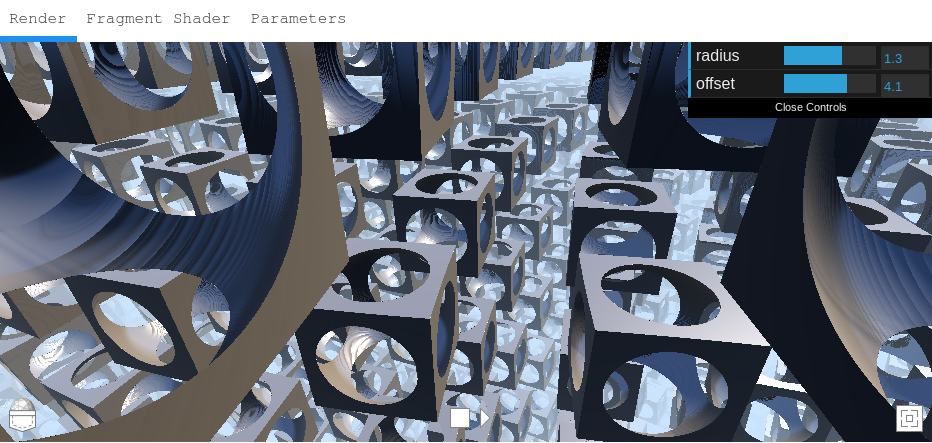
\includegraphics[width=\textwidth]{screenshot_sphere_tracing.png}
  \caption{Render from sphere tracer used in project}
  \label{fig:sphere tracer}
\end{figure*}

Like the prior chapter, this distance function representation is used
to express some basic shapes.  This is then used as the basis to
express some rigid body 3D transformations via matrices and then via
quaternions; this is then generalized to the same sorts of domain
transformations that were done in the 2D case.

\section{Limitations, Problems \& Future Work}

This work is considered to be some mix of a draft and a
proof-of-concept.  Besides minor bug-fixes and features in the
environment itself, it has several areas for further improvement.

The content covered a limited scope of mathematical topics, mostly due
to time constraints.  It could, and perhaps should, extend to further
topics that can be explained similarly.  To name a few that were
planned but not completed, the content was supposed to also include
eigendecompositions, matrix inverses, fractals, and iterated function
systems.  The entire fourth chapter (at least, at the time of this
writing) of the content contains a list of references to further
topics which might sensibly be integrated in.  The content also
presently doesn't have the benefit of much feedback from people who
attempted to learn from it.

Also due to time constraints, parts of the environment itself were
adapted from existing libraries rather than being written from
scratch.  Some of these might more sensibly be rewritten from scratch
(or at least something lower-lever).  In somewhat the opposite way,
some other parts that were written by hand might be better off
replaced with a separate module.  To name one, the project could
perhaps employ \href{https://github.com/stackgl/glslify}{glslify} to
assist with the very ad-hoc management of packages presently in used
in the environment's WebGL code.

The environment is also somewhat coupled to WebGL right now.  Making
the WebGL support more of a separate module may make this more useful
to extend to other languages that might run in the browser.

Features were planned which would give the environment more of a
``social'' nature, such as the one provided in Scratch.  The authors
of Scratch distilled its design philosophy down to, ``Make it more
tinkerable, more meaningful, and more social than other programming
environments.''\cite{Resnick2009} and spoke extensively of the
importance of social networks in education.  None of these features
were implemented, however, environments like Scratch,
\href{https://www.shadertoy.com/}{ShaderToy}, and
\href{https://www.openprocessing.org/}{OpenProcessing} give some ideas
for what form these might take.

\bibliographystyle{ACM-Reference-Format} \bibliography{chodapp3_final_paper,chodapp3_final_paper_mendeley}

\end{document}
